\section{Implementation}\label{sec:implementation}

\begin{figure}[H]
\centering
\begin{minted}{python}
def satisfiable(p: Proposition, backend_or_sampler, is_backend: bool) -> bool:
    oracle, atom_lookup = phase_oracle(p)
    grover_op = grover(oracle, atom_lookup)
    N = 2 ** count_atomic_propositions(p)
    m = 1
    while m <= math.sqrt(N):
        k = random.randint(1, round(m))
        grover_k_times = QuantumCircuit(grover_op.num_qubits)
        grover_k_times.h(list(range(len(atom_lookup))) + [grover_op.num_qubits - 1])
        for _ in range(k):
            grover_k_times.compose(grover_op, inplace=True)
        grover_k_times.measure_all()
        if is_backend :
            grover_k_times = transpile(grover_k_times, backend_or_sampler)
            result = (
                backend_or_sampler.run(grover_k_times, shots=1).result().get_counts()
            )
        else:
            result = backend_or_sampler.run([grover_k_times], shots=1).result()[0].data.meas.get_counts()
        result_bit_string = next(iter(result))[::-1]
        witness_assignment = {}
        for atom in atomic_propositions(p):
            witness_assignment[atom] = char_to_bool(
                result_bit_string[atom_lookup[atom]]
            )
        if valuation(p, witness_assignment):
            return True
        m = (5 / 4) * m
    return False
\end{minted}
\caption{Implementation of \mintinline{python}{satisfiable} }
\label{fig:satisfiable}
\end{figure}

\subsection{\texttt{phase\_oracle} Implementation}

\autoref{fig:oracle} should give an idea of the circuit that \texttt{phase\_oracle} returns, however, there are some differences: The circuit produced by \texttt{phase\_oracle} only has one output bit, and the result is encoded in the phase instead of the bit.
This is done because the \texttt{GroverOperator} function, provided by Qiskit, expected such a circuit.

\begin{figure}[H]
    \centering
    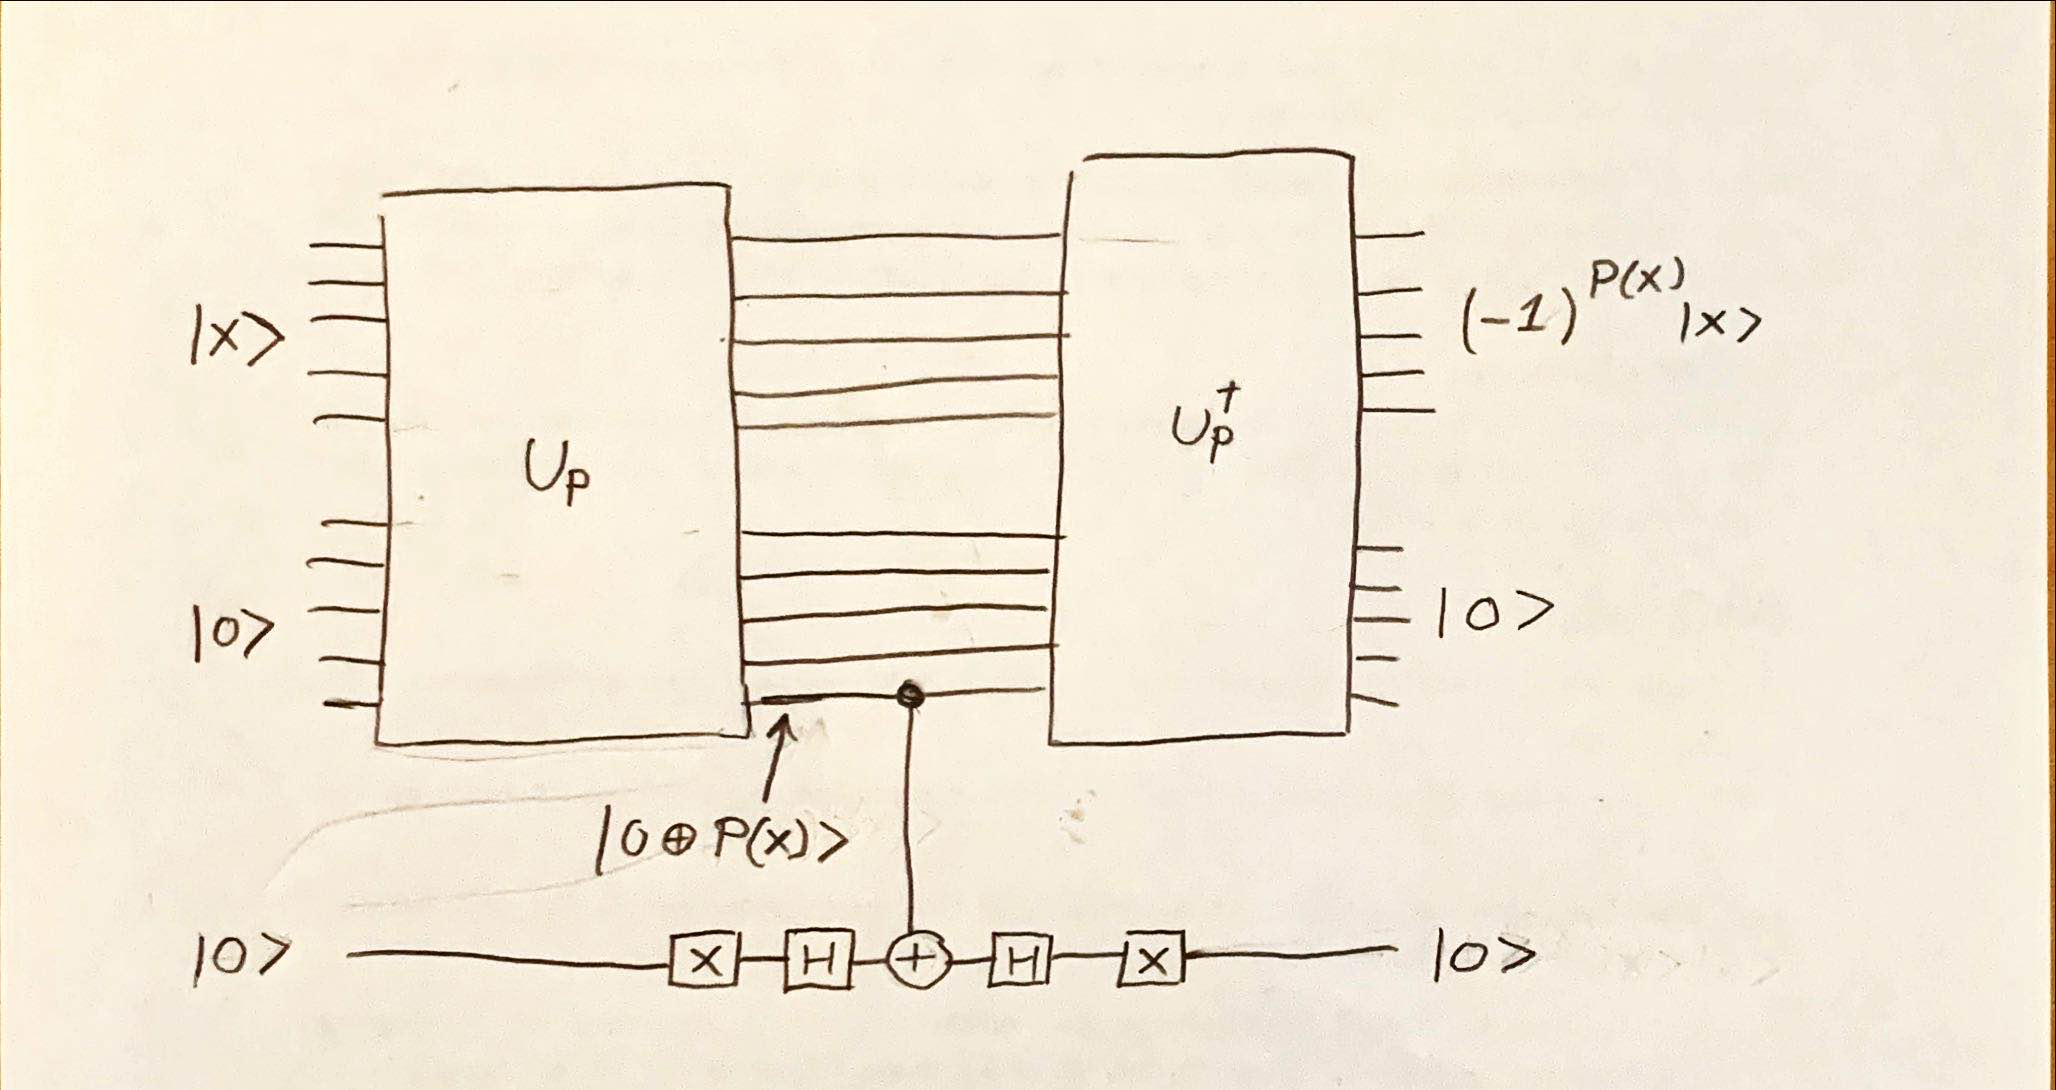
\includegraphics[width=\textwidth]{figures/garbage-free-computation.jpg}
    \caption{Oracle circuit}
    \label{fig:oracle}
\end{figure}

First off, on line 1, a lookup table relating atomic propositions to their location inside the circuit is created.
This lookup table is returned along with the circuit.
Further, in line 2, the base circuit where qubits corresponding to atomic propositions reside is created.
On line 3, the circuit $R$ is created, this is further described in \autoref{subsubsec:phase-oracle-recur-implementation}.
On line 6 through 12 the result is encoded in the phase of a separate qubit, by sandwiching a controlled not gate, depending on the result of $R$, between a not and Hadamard gate.
Finally, on line 13 through 15, $R^\dagger$ is created and added to the circuit, and the circuit and lookup table are returned.

\begin{figure}[H]
\centering
\begin{minted}{python}
def phase_oracle(p: Proposition) -> Tuple[QuantumCircuit, Dict[str, int]]:
    atom_lookup = {item: index for index, item in enumerate(atomic_propositions(p))}
    qc_base = QuantumCircuit(len(atom_lookup))
    qc_r = phase_oracle_recur(p, qc_base, atom_lookup)
    qc_r_r_daggert_pos = list(range(0, qc_r.num_qubits))
    qc_final = QuantumCircuit(qc_r.num_qubits + 1)
    qc_final.compose(qc_r, qc_r_r_daggert_pos, inplace=True)
    qc_final.x(qc_final.num_qubits - 1)
    qc_final.h(qc_final.num_qubits - 1)
    qc_final.cx(qc_final.num_qubits - 2, qc_final.num_qubits - 1)
    qc_final.h(qc_final.num_qubits - 1)
    qc_final.x(qc_final.num_qubits - 1)
    qc_r_daggert = qc_r.inverse()
    qc_final.compose(qc_r_daggert, qc_r_r_daggert_pos, inplace=True)
    return qc_final, atom_lookup
\end{minted}
\caption{Implementation of \mintinline{python}{phase_oracle} }
\label{fig:phase_oracle}
\end{figure}

\subsubsection{\texttt{phase\_oracle\_recur} Implementation}\label{subsubsec:phase-oracle-recur-implementation}

\subsection{\texttt{grover} Implementation}

\begin{figure}

\end{figure}

\begin{figure}
\centering
\begin{minted}{python}
def grover(oracle: QuantumCircuit , atom_lookup: Dict[str, int]) -> QuantumCircuit:
    qc_state_prep = QuantumCircuit(oracle.num_qubits)
    qc_state_prep.h(oracle.num_qubits - 1)
    for i in range(len(atom_lookup)):
        qc_state_prep.h(i)
    reflection_qubits = list(range(len(atom_lookup))) + [oracle.num_qubits - 1]
    grover_op = GroverOperator(
        oracle, qc_state_prep, reflection_qubits=reflection_qubits
    )
    return grover_op
\end{minted}
\caption{Implementation of \mintinline{python}{grover} }
\label{fig:grover}
\end{figure}
